\documentclass{article}
\usepackage[utf8]{inputenc}
\usepackage{xcolor}
\usepackage{amsmath}
\usepackage{scrextend}
\usepackage{listings}
\usepackage{tcolorbox}
\usepackage{graphicx}
\usepackage{tikz}
\usepackage{float}
\usepackage{hyperref}
\setlength{\parindent}{0pt}
\setlength{\parskip}{12pt}
\setlength{\intextsep}{0pt plus 2pt}
\usepackage{multicol}
\usepackage{tikz}
% For setting margins
\usepackage[margin=2in]{geometry}
\definecolor{darkgreen}{RGB}{50,150,50}
\definecolor{darkred}{RGB}{150,50,50}

\def\checkmark{\tikz\fill[scale=0.4, color=darkgreen](0,.35) -- (.25,0) -- (1,.7) -- (.25,.15) -- cycle;} 
\def\crossmark{\tikz\draw[scale=0.4, color=darkred, line width=0.3mm](0,0) -- (.5,.5) -- (0.25, 0.25) -- (0,0.5) -- (0.5, 0);} 

\graphicspath{{.}}

\title{DD2360 GPU Architecture}
\author{Jonas Valfridsson\\ 199608275377}

\begin{document}

\maketitle

\subsection*{Exercise 1}%
\label{sub:exercise_1}



\subsubsection*{Why GPUs emerged as suitable hardware for computer graphics?}%
\label{ssub:why_gpus_emerged_as_suitable_hardware_for_computer_graphics_e_g_games_}

Because many of the tasks in computer graphics are 'ridiculously parallel' meaning you get a linear performance boost by increasing the number of cores the
program runs in. Consider Ray-tracing, you need to trace a ray for each pixel on your screen, the result for each pixel are independent of the computations
of other pixels: meaning they can be computed completely in parallel. Therefore adding extra cores to a ray-tracing engine will linearly boost its performance.
GPU's advantage is that they pack many cores. Therefore since computer graphics benefits from having many cores and it is what GPUs have: GPUs emerged as suitable
hardware for that task.

\subsubsection*{Why do we talk about throughput-oriented architecture when we talk about GPUs?}%
\label{ssub:_why_do_we_talk_about_throughput_oriented_architecture_when_we_talk_about_gpus_}

Because we are optimising for the throughput of many parallel tasks rather than the performance of one single serial task. Continuing on the ray-tracing example:
we are more concerned with being able to trace more pixels per unit of time than having tracing a single pixel take less time.

To clarify, GPU's try to maximize the total throughput of all tasks at the risk of some increased latency for individual tasks. Because in the end the problem we
try to solve with GPU's are more concerned with the total throughput.

\subsubsection*{List the main differences between GPUs and CPUs in terms of architecture.}%
\label{ssub:}

\begin{itemize}
  \item GPU's have many cores 
  \item CPU's have fewer cores
  \item GPU's have a topology of cores that is good for distributed computations 
  \item Because of GPU's core topology they tend to be fat blobs, wide and shallow
  \item CPU's focus on finishing tasks on their cores quickly, this is good for serial computations 
  \item CPU's tend to be more narrow and deep.
\end{itemize}

Some worthwhile differences to mention is that CPU cores tend to have much bigger caches, higher clock speed and perform additional single core optimisations to
make single programs run faster e.g branch prediction. 

\subsubsection*{My GPU specs}%
\label{ssub:my_gpu_specs}

I have access to two different GPU's that I might be using during this course, first

% Answer number of SMs (Streaming multiprocessors), number of cores per SM, clock frequency, memory size.

\textbf{GPU on Nvidia Jetson Nano \cite{Jetson-Nano}}: 

\begin{itemize}
  \item Each SM has 32 Cuda cores
  \item 128 Cores in Total
  \item 4 SM's
  \item Clock Speed 640 MHz
  \item 4GB memory
\end{itemize}

And then my desktop GPU:

\textbf{Nvidia 1080 GTX TI \cite{1080ti}}: 

\begin{itemize}
  \item Each SM has 128 Cuda cores
  \item 3584 Cores in Total
  \item 28 SM's
  \item Clock Speed 1582 MHz
  \item 11GB memory
\end{itemize}


\subsubsection*{The New Nvidia GPU's}%
\label{ssub:the_new_nvidia_gpu_s}



\textbf{Which Operation does the \textit{Tensor Core} support in one cycle?}%


It doing a GEMM per cycle.  GEMM stands for '\textbf{GE}neralized \textbf{M}atrix \textbf{M}ultiplication'.

\textbf{What is the Precision supported by Tensor Cores?}%

The latest generation supports TF32, bfloat16, FP16, INT8, INT4 and it seems to also now support FP64 \cite{tensorprecision}

\textbf{Why do you think that Tensor Cores were introduced in the new GPUs?}%

Applications based on matrix multiplications have grown increasingly popular, e.g machine learning. Building custom operations for these applications was a good
idea. I think they were introduces into GPU's partly to accelerate machine learning tasks.

\textbf{What are the differences between GPUs with Tensor cores and TPUs?}

Not much.. 

The TPU uses Matrix Multiply Units that is made up of some topology of MAC's (256x256) that can perform 8bit signed and unsigned multiply-and-add, the matrix
unit can perform either a matrix multiplication or a convolution in one clock cycle. \cite{jouppi2017datacenter}

Each tensor core in a GPU can perform a 'matrix-multiply-and-accumulate' on 4x4 matrices per clock cycle - using mixed precision. \cite{nvidiatensorcores}

So some initial differences is the precision that the hardware is working with. The second is that the TPU s made out of bigger computational
blocks, e.g each Matrix Multiply Unit is made of (256x256) MAC's. The TPU also supports a single clock cycle convolution operator. 

Both devices are similar in that they support single-cycle matrix operations, but they differ in size of their computation units. TPU's were for example designed
specifically for dense operations, they do not support sparse operations very well.


\textbf{Which operation does the Nvidia Ray Tracing core support in one clock cycle?}

The RT core contains two specialized units: one that does bounding box tests and one for ray-triangle intersection testing. Basically the RT core implements an
instructions that can check if a ray has hit a primitive or not using the BVH.

\subsubsection*{How many of the top 10 most powerful supercomputers use GPUs?}%
\label{ssub:}



\begin{enumerate}
  \item Supercomputer Faguku \crossmark
  \item Summit \checkmark
  \item Sierra \checkmark
  \item Sunway TaihuLight \crossmark
  \item Tianhe-2A \crossmark
  \item HPC5 \checkmark
  \item Selene \checkmark
  \item Frontera \checkmark
  \item Marconi-100 \checkmark
  \item Piz Daint \checkmark
\end{enumerate}

\subsubsection*{Use Google Scholar to find a scientific paper reporting about a work using GPUs in your main domain area}%
\label{ssub:use_google_scholar_to_find_a_scientific_paper_reporting_about_a_work_using_gpus_in_your_main_domain_area}


I pick the 'Attention is all you need' paper from Google. It was published in NIPS 2017, the authors are the following: Ashish Vaswani, Noam Shazeer, Niki
Parmar, Jakob Uszkoreit, Llion Jones, Aidan N. Gomez, Łukasz Kaiser, Illia Polosukhin. They used 8 P100 GPUs to train a NLP model, the programming was done
using Tensorflow, a High level library for machine learning that makes use of cuda, cudNN and tensorRT to accelerate itself on GPUs.




\subsection*{Exercise 2}%
\label{sub:exercise_2}


Running ./bandwidthTest on my desktop GPU gives

\begin{lstlisting}[language=bash]
[CUDA Bandwidth Test] - Starting...
Running on...

 Device 0: GeForce GTX 1080 Ti
 Quick Mode

 Host to Device Bandwidth, 1 Device(s)
 PINNED Memory Transfers
   Transfer Size (Bytes)        Bandwidth(MB/s)
   33554432                     6525.9

 Device to Host Bandwidth, 1 Device(s)
 PINNED Memory Transfers
   Transfer Size (Bytes)        Bandwidth(MB/s)
   33554432                     6501.7

 Device to Device Bandwidth, 1 Device(s)
 PINNED Memory Transfers
   Transfer Size (Bytes)        Bandwidth(MB/s)
   33554432                     60001.2

Result = PASS

\end{lstlisting}

Running ./bandwidthTest --mode=shmoo on my desktop GPU gives

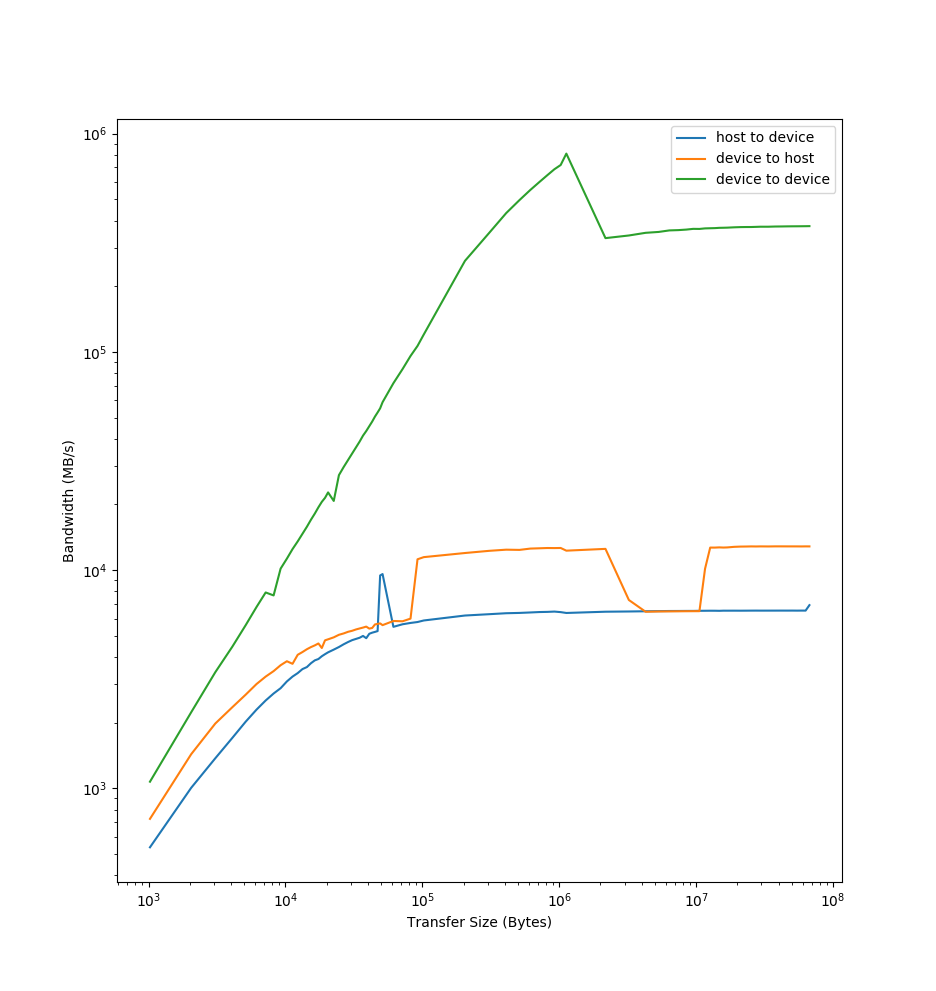
\includegraphics[scale=0.5]{devices.png}

Device to device is much faster, as expected, since we are not bottlenecked by between-device communication.

The reason why device to device communication increases linearly for longer than between device communication is for the same reason, the bandwidth on within
device communication is larger so it supports greater information transfer, while between device communication bottlenecks earlier.




  




\begin{thebibliography}{1}

\bibitem{Jetson-Nano} Hardware information of the Jetson Nano -
  \href{https://developer.download.nvidia.com/assets/embedded/secure/jetson/Nano/docs/JetsonNano_DataSheet_DS09366001v1.0.pdf?iaSvUlG13V9tO_rXL4A6TSmWGgvF2rSYMQNAA7H0PGswJ3Ce29p9QHbgqQYfW539zMaLP0UgEZ4sk1uQuZyNt_27VZofFR1NN5A0AFbZ2ZgMVtxj01KRbMQBTwmpzEvydG9r0NRMDTGXC75N0W2yAn2pO9rc-qiop05-HERWP5O6ACDsok9m7cfYjxUlxQ}{link}
\bibitem{1080ti} Link to 1080ti homepage: \href{https://www.nvidia.com/en-sg/geforce/products/10series/geforce-gtx-1080-ti/}{link}
\bibitem{tensorprecision} Link to nvidia page: \href{https://www.nvidia.com/en-us/data-center/tensor-cores/}{link}
\bibitem{jouppi2017datacenter} {\textbf{In-datacenter performance analysis of a tensor processing unit}}, {Jouppi, Norman P and Young, Cliff and Patil, Nishant and Patterson, David and Agrawal, Gaurav and Bajwa, Raminder and Bates, Sarah and Bhatia, Suresh and Boden, Nan and Borchers, Al and others}, {2017}
\bibitem{nvidiatensorcores} \textbf{NVIDIA Tensor Core Programmability, Performance \& Precision} 2018 IEEE International Parallel and Distributed Processing Symposium Workshops

\end{thebibliography}

\end{document}




